% Design Development 
\chapter{Design Development}
\label{sec-development}

For fall, the development chapter focuses on benchmarking, need-finding, persona development and the first critical function and critical experience prototypes. For later quarters, many of these details will go to an appendix, with just a summary of the main findings and insights. Even in fall, the focus should be on findings and lessons learned.

\begin{remark}  \color{blue}
\begin{itemize}\tightlist
\item Focus on results (e.g., key findings, insights, lessons learned), not team activities (``We brainstormed extensively and eventually settled on two alternative concepts.'')
\item Use lots of images, and not just photographs: diagrams, schematics, flow charts, CAD renderings, etc. are often much more informative than a photo. In any case, use labels pointing to the features you want the reader to appreciate. Also, do refer to all of your figures explicitly in the  text (\emph{As shown in figure xx, ... }).
\item Lengthy details (e.g. detailed results of technical benchmarking) should go in an Appendix section, with an explicit forward reference from this section. In winter and spring, much of this material will go to an appendix.
\item Be professional: it's essential to properly cite sources of information and provide credits for any images you are using that you did not generate yourselves.
\item Don't refrain from describing ideas that were briefly pursued and dropped. Explain why they were abandoned. In other circumstances they might be worth picking up again.
\item You can use tools such as Pugh concept selection, function-structure diagrams and design decomposition 
\cite{Otto07,OttoWood01,UlrichEppinger95} to organize and clarify your design process. Many web-based tools also exist for diagramming relationships (e.g. \url{http://vue.tufts.edu} ). A nice side-effect is that such diagrams help with documentation.
\end{itemize}

The remaining text in this section contains excerpts from the Autodesk 2007-08 Fall document \cite{Autodesk2008Fall} and some additional explanatory examples.
\normalcolor 
\end{remark}

We drew from our diverse individual experiences to redefine the problem as we learned more about existing collaborative tools and practices. Throughout the design development process, shown in figure \ref{fig:Design_Development_Flowchart}, we balanced pushing forward with our current ideas while looking for new directions. 

\begin{figure}[h]
\centering
		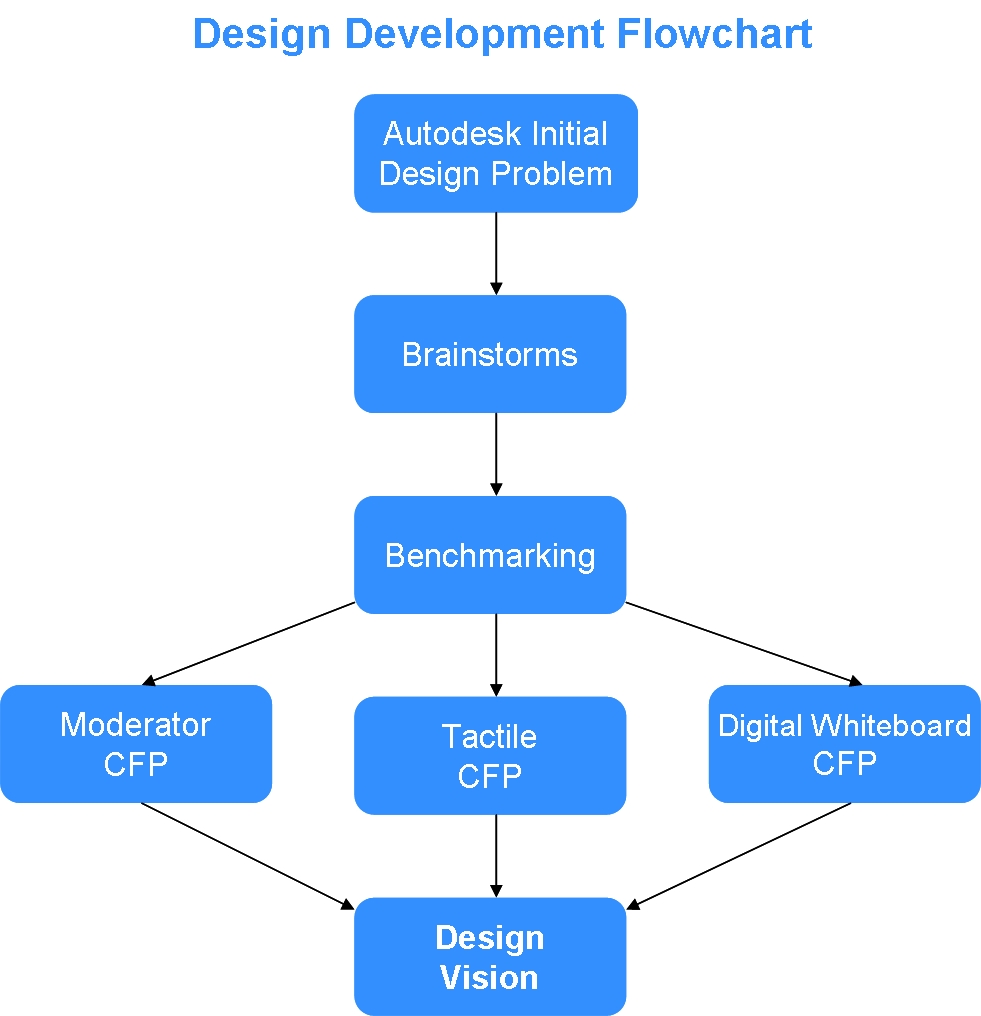
\includegraphics[keepaspectratio, width=4in]{Figures/Ch4/Design_Development_Flowchart.jpg}
	\caption{The design team's development process.}
	\label{fig:Design_Development_Flowchart}
\end{figure}

\section{Brainstorming}
\label{sec:brainstorm}

	Our experience in brainstorming was unique in that we were observing and studying our own behavior while exploring solutions. We were constantly studying our own triumphs and shortcomings in the hopes of gaining insight into team dynamics. The results of our multiple brainstorms throughout the fall quarter can be into categorized the following categories:

\subsection{Communication}

\begin{figure}[h] 
\centering
		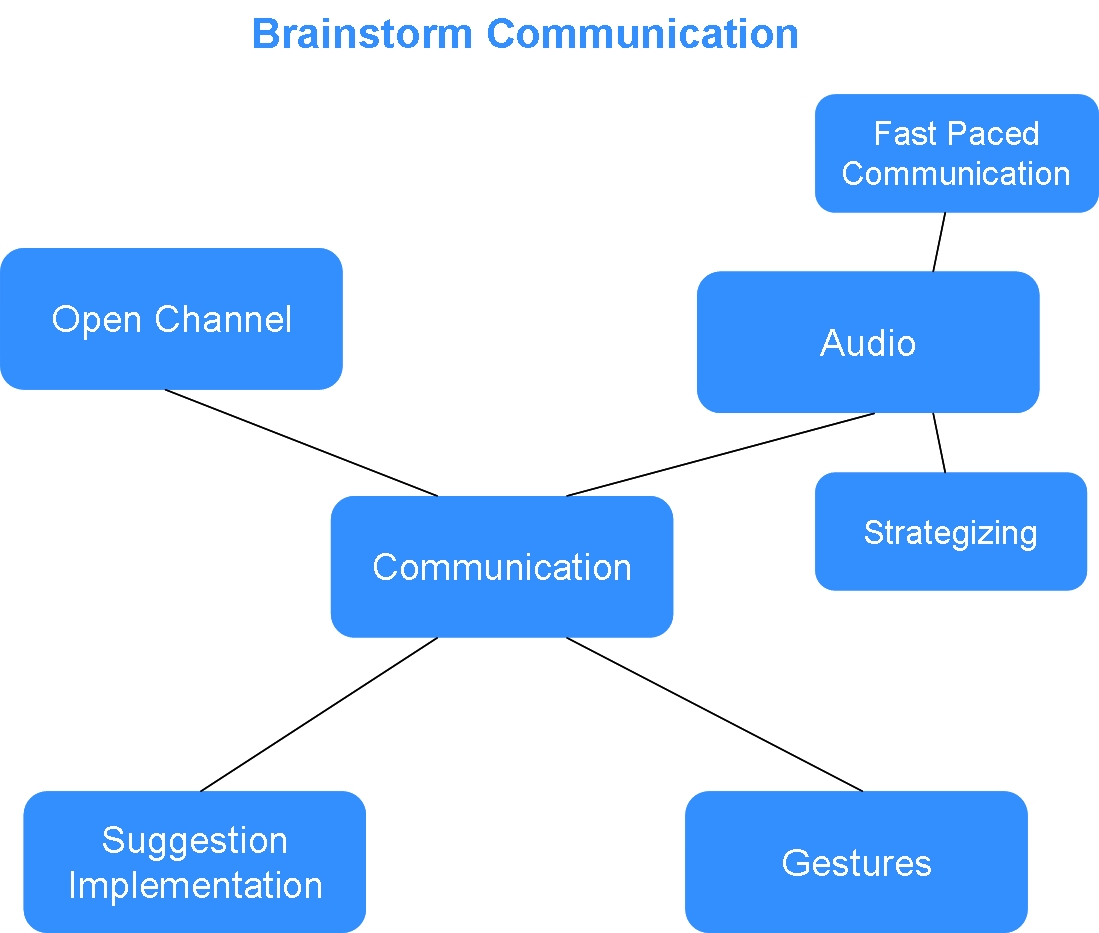
\includegraphics[keepaspectratio, width=3in]{Figures/Ch4/Brainstorm_Communication.jpg}
	\caption{Key components of communication in design meetings}
	\label{fig:Brainstorm_Communication}
\end{figure}

\begin{itemize} \tightlist 
\item {Open channels}
\item \begin{itemize} \tightlist Audio and video channels are often inundated with information, even if they are not the most effective means to transmit a piece of information. The team learned that messages are most clearly conveyed when they are free from interference. \end{itemize}
\item Integrate suggestions quickly
\item \begin{itemize} \tightlist People can build onto other's ideas immediately, and rapidly change the direction of the conversation. \end{itemize}
\item \textbf{Verbal communication is the most flexible}
\item \begin{itemize} \tightlist The team learned from their experience playing cutting-edge multiplayer videogames that verbal communication was the most relied upon medium during fast and slow paced activities. It's versatility and low-bandwidth warranted future attention. \end{itemize}
\item Gesture
\item \begin{itemize} \tightlist Gesture is frequently used when explaining an idea. Often, the drawings produced do not look at all like the concept being developed, but the act of drawing in and of itself can be like a gesture, showing how something will work, or where it will be placed, and so forth. \end{itemize}
\end{itemize}

\begin{center}
\emph{The rest of this subsection is omitted for brevity}
\end{center}

Some key realizations from the brainstorming phase were that social factors and communication shortcomings had alot of opportunity for development. We decided to give special attention to social benchmarking in addition to our technological research.

\section{User benchmarking and need-finding}
\label{sec:needfinding}

In this section briefly describe activities undertaken to come to an understanding of users or potential users and their needs. An important part of this section is the development of personas.

\subsection{Personas development}
\label{sec:personas}

Describe the personas, what findings are incorporated in them, and what insights they provide for the design.  Ideally include some images of your personas, like ``Kevin'' in figure \ref{fig:personakevin} from the 2011 Lockheed project \cite{LockheedMartin2011}.

\begin{figure}[h]
\centering
		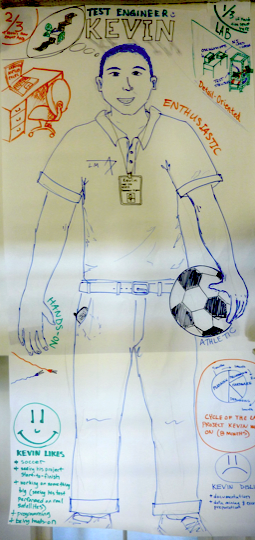
\includegraphics[keepaspectratio, width=2in]{Figures/Ch4/persona-kevin.png}
	\caption{A persona for a satellite testing project (from \cite{LockheedMartin2011})}
		\label{fig:personakevin}
\end{figure}

\section{Business Benchmarking}

A recent element in me310-global thinking process is to be explicitly aware of the client's business model.  
The motivation for this new element is our growing awareness that coming up with the next ``big-idea'' may be the easy part of our quest.  The harder part may be gaining acceptance of our break-through innovation within the organization. 
Please be aware that the canvas can be re-organized to suit your situation. 

A starting point could be the ``Business Canvas Model''
introduced in class (figure \ref{fig:businesscanvas}) with reference to
\cite{osterwalder2010business} for more background information.

Bencharking the corporate partner's business model and goals is part of benchmarking, and can be covered in a section 
in this design development chapter. Some examples of recent ME310 documents with fairly extensive business
benchmarking include the 2012 Spring documents from Electric Mobility Norway \cite{EMN2012Spring} and Symbiose\'{e} \cite{Symbiosee2012Spring}.

\begin{figure}[ht]
\centering
		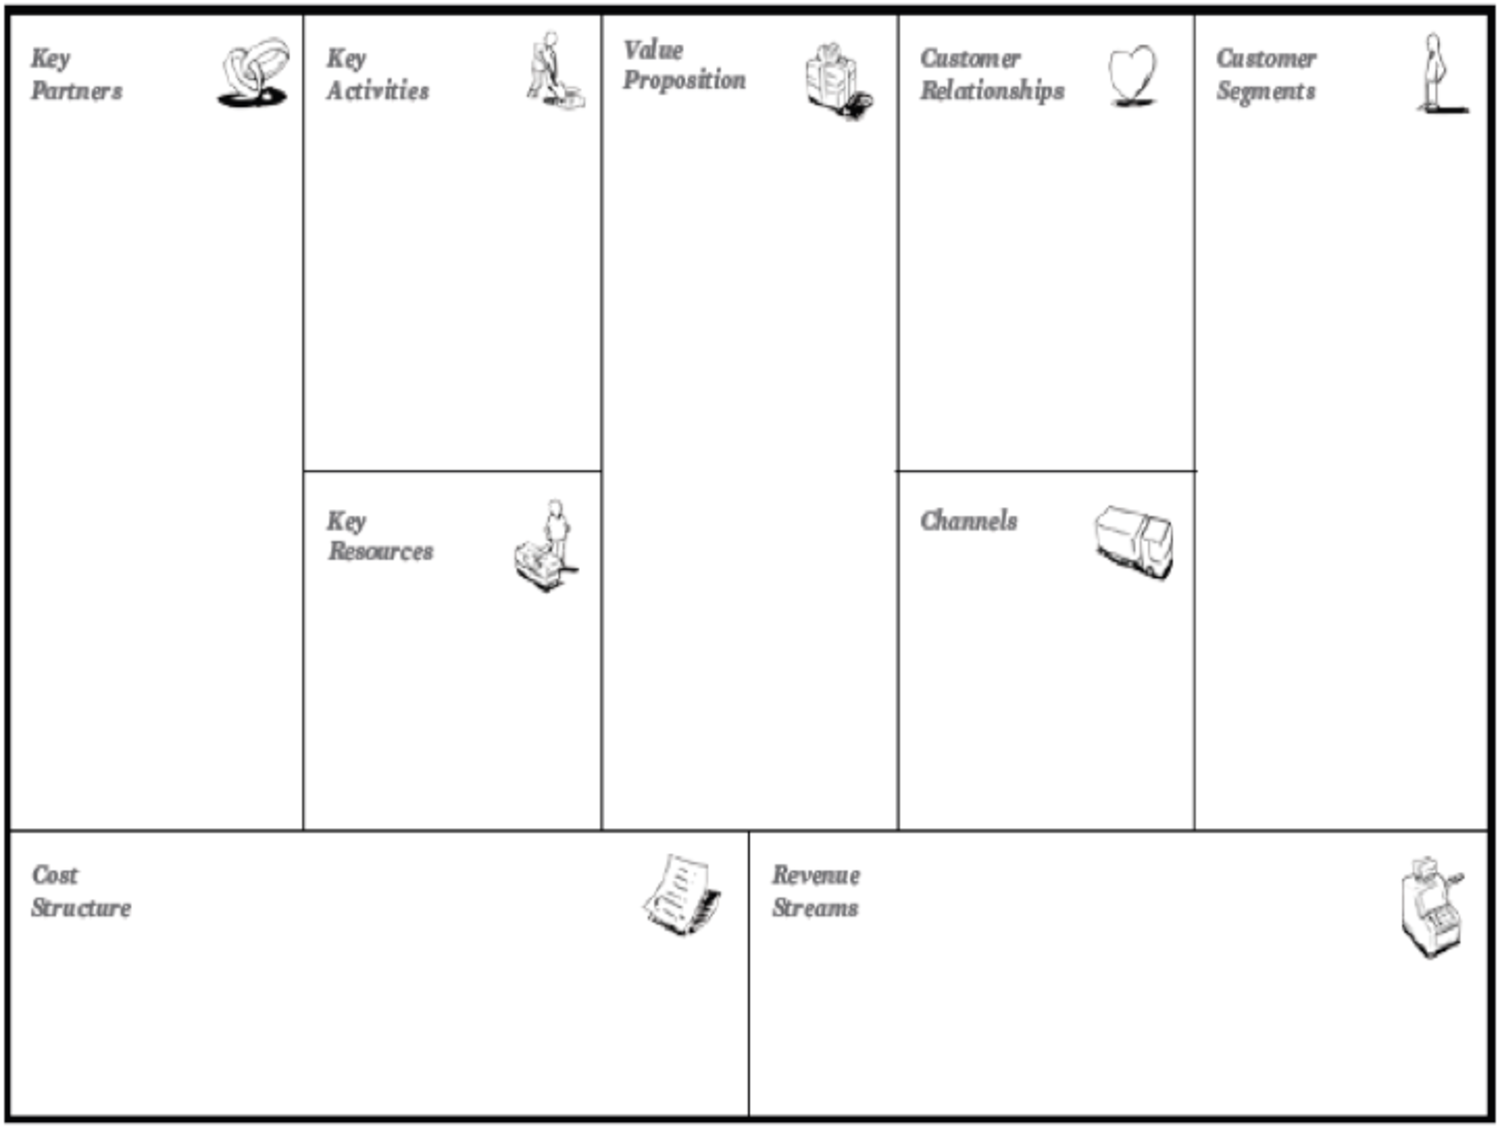
\includegraphics[keepaspectratio, width=4in]{Figures/Ch4/BusinessCanvas.pdf}
	\caption{Business Canvas (from \cite{osterwalder2010business}).}
		\label{fig:businesscanvas}
\end{figure}


\section{Technology benchmarking}

	The team's research and benchmarking efforts were focused on three major categories: human-machine interfaces and input devices, social dynamics, and communication. The methods the team utilized to research items in these three main categories  included trying out hardware, drawing on previous experience, participating in improv exercises, researching existing solutions, and speaking to experts from design, neuroscience, and computer science.
	
\subsection{The Nintendo Wii - Accelerometer-based input)}

\begin{figure}[h] 
\centering
		\includegraphics[keepaspectratio, width=4in]{Figures/Ch4/Wii.jpg}
%Note the use of a short caption tag for the list of figures.
	\caption[Nintento Wii]{People playing Wii Sports on the the Nintendo Wii.
	\color{blue}There should be a citation to the URL this photo came from\normalcolor. }
\end{figure}

	The team investigated some unconventional means for data input. Gesture-based input devices like the Nintendo Wii controller offer the possibility of an intuitive, and compelling way to interact with someone at distance via digital means.  For navigating through Windows or other applications, the team found the Wii to be  more challenging than a conventional mouse.  Accelerometers are adept at capturing large motions rather than precision pointing and would need to be utilized as such. Potential applications could be for interfacing with avatars or tactile feedback systems. The Wii controller could be used as a gesture-based communication device to control a personal avatar or send and receive tactile messages.
	
\noindent \textbf {Key lessons learned}
\begin{itemize} \tightlist 
\item Accelerometer based input devices could be used in gesture-based or tactile communication, but do not fare well in precision pointing.
\item Gesture-based interfaces generate excitement. People want to use input devices that respond to gesture. 
\end{itemize}

\subsection{CyberGlove \textregistered}

\begin{figure}[h] 
\centering
		\includegraphics[keepaspectratio, width=4in]{Figures/Ch4/CyberGlove.jpg}	
%Note the use of a short caption tag for the list of figures.
	\caption[Cyberglove]{CyberGlove gesture-based input device. \color{blue}There should be a citation to the URL this photo came from\normalcolor.}
\end{figure}

\begin{center}
\color{blue}
The rest of this subsection is omitted for brevity
\normalcolor
\end{center}

\subsection{EEG and Participation Monitor}

\begin{figure}[h] 
\centering
		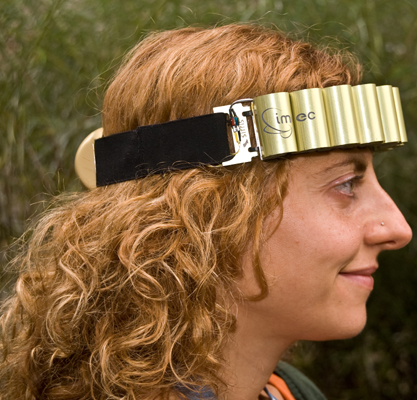
\includegraphics[keepaspectratio, width=3in]{Figures/Ch4/EEG.jpg}
	\caption[Wireless EEG]{Example of the first available wireless EEG tool, made by IMEC. \color{blue}There should be a citation to the URL this photo came from\normalcolor.}
\label{fig:wirelessEEG}
\end{figure}

	The team met with Alicia Warlick, a researcher in the Stanford Neuroscience Department, and her research in monitoring brainwaves. We discussed the possibility of monitoring whether meeting participants were actively paying attention by using an EEG. This is a method for measuring the activity level of the brain. There is opportunity to use this as a metric for testing our final product, or potentially in the product itself as a means to collect data on user participation level.

\noindent \textbf{Key lesson learned}
\begin{itemize} \tightlist
\item  Electrodes could be placed on the users forehead and scalp (as in Fig. \ref{fig:wirelessEEG}) to measure EEG readings, which conveys information about whether someone is engaged in what they are doing, or if they are withdrawn.
\end{itemize}

\begin{center}
\color{blue}
The rest of this subsection is omitted for brevity
\normalcolor
\end{center}

%%%%%%%%%%%%%%%%%%%%%%%%%%%%%%%%%%%%%%%%%%
%This starts a major new subsection on the final CFP and CEP of Fall quarter, so
%probably makes sense to put in a clearpage command to let figures catch up.
\clearpage

\section{Critical Function and Critical Experience Prototypes (CFP/CEP)}
	The initial benchmarking phase lead the team to realize that there were three major challenges to solve: bridging the proximity gap, moderating brainstorming, and conveying and recording ideas. The team decided to tackle all three of these major challenges and designed four CFPs in an attempt to solve, or at least start answering some of, the questions these challenges brought up. 

\subsection{Tactile CFP}

The team wanted to come up with a creative solution that would enhance distance communication. Although we identified software having an important role in our solution, we wanted to try to design something physical. We had to answer these questions that were raised after the benchmarking process:
\begin{itemize} \tightlist
\item How can we simulate proximity for remote meetings?
\item How can we implement action-event control?
\item What senses can we stimulate that aren't normally used?
\item What is a low bandwidth solution?
\end{itemize}

	The team decided that building a tactile messaging system would solve all four of the aforementioned questions. Tactile messages could replace common interpersonal interaction found in same room meetings. It is normal to welcome each other with a  handshake, make eye contact throughout a meeting, smile at each other, and give high-fives to congratulate others. These occurrences are all absent from distance meetings. A tactile message corresponding to each of these gestures would allow users similar opportunity to communicate as if they were sharing the same physical meeting room.
	
	The team learned that immersive activities like videogames take advantage of action-event control to offer users a seamless means to interact with their environment. A tactile message could quickly be sent over an open channel and pressing the �on� button would instantly message the recipient.
	
	Out of the five senses (sight, hearing, taste, touch, and smell), sight and hearing are the most relied upon during meetings. The team considered possibilities in taste and smell messaging but continued with touch, since delivery of tactile messaging was much more straightforward. Since conventional distance meetings only send and receive auditory and visual information, tactile messages would be distinct and easy to identify. The team believed that tactile messages (high, low, or off) would be low bandwidth.

	\begin{figure}[h] 
\centering
		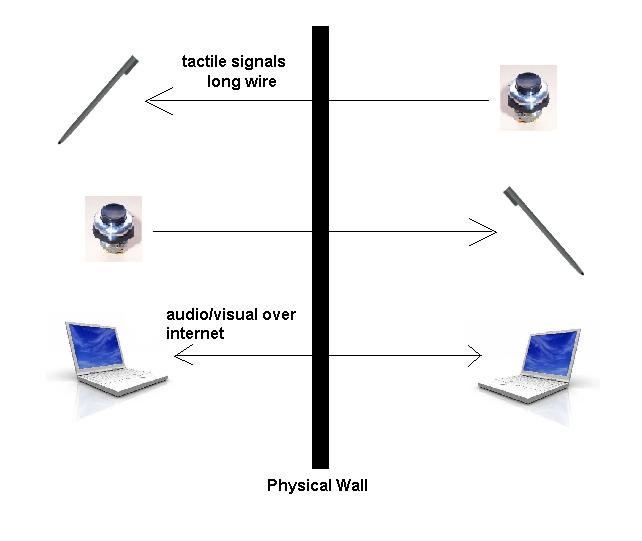
\includegraphics[keepaspectratio, width=4in]{Figures/Ch4/tactileCFPschematic.jpg}
	\caption{The team's whiteboard during a brainstorm session}
\end{figure}

	The team wanted to test the effectiveness of tactile messaging and decided against a TCP/IP protocol that sent messages between Stanford and PUJ. The code to write such a protocol was extant and it was unnecessary to include it in our prototype. The team simplified the setup and created two stations separated by physical barriers (a wall and 50' of distance), to simulate a distance meeting. Each station would have a vibrating tactile device for each seated participant at that station and a high/low button assembly to activate the vibrating tactile device for each participant at the other station. Initially the devices were supposed to operate as ''on'' or ''off.'' The team decided that having more variability in the operating speeds of the motors would increase the number of different messages that could be sent, and added a high and low voltage button (1.2V and 0.6V).
	
	We were curious to see if effective communication could take place if a distant colleague could see what sketches his distant colleague was drawing. To test this, we used webcams to send live video of what the participants drew on their drawing pads to the other stations.

\subsubsection{What is critical about this CFP?}
	The team identified these questions as critical before testing:
\begin{enumerate} \tightlist
\item Can it create immersion?
\item Does it improve upon existing communication tools?
\item Is it easy to understand?
\item Is it intuitive?
\item When should it be used?
\end{enumerate}

\begin{figure}[h] 
\centering
		\includegraphics[width=3in]{Figures/Ch4/tactile_seating.jpg}
	\caption{The orientation of the two tactile messaging stations.}
\end{figure}

\subsection{Tactile Messaging CFP Description}

The remaining text in this section contains of excerpts from the Autodesk 2007-08 Fall document \cite{Autodesk2008Fall}.

The tactile messaging system was comprised of small Jameco vibrating motors (1.3VDC 8,500 RPM) mounted to ball point pens and wrist patches. A simple switchable voltage supply circuit was created to give each vibrating motor a high (1.2V) and low (0.6V) vibrating speed (\ref{fig:tactile_circuit}). Each voltage level was buffered with LM324 opamps, and the circuits were implemented on protoboards. The high and low speeds were selected by switches. 

\begin{figure}[bhtp] 
	\begin{center}
		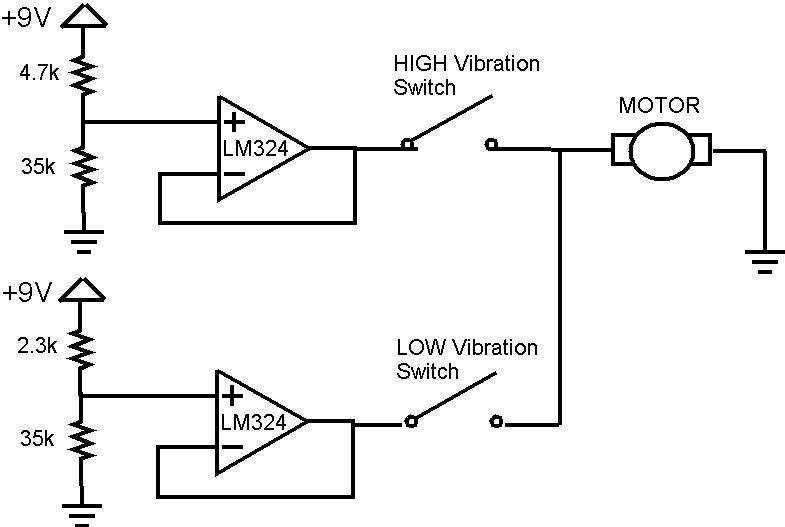
\includegraphics[width= \figwidth]{Figures/Ch5/tactile_circuit.jpg}
	\end{center}
	\caption[voltage divider]{A simple voltage dividing circuit provided 1.2V (HIGH) and 0.6V (LOW) buffered output voltages for the vibrating motor. Switches triggered the high and low voltages. }
	\label{fig:tactile_circuit}  
\end{figure}

\begin{center}
\color{blue}
(Text omitted for brevity)
\normalcolor
\end{center}

Four independent circuits were created to provide messaging to two motors on each side. 90' 16-gauge wire was passed between two stations in the meeting setup shown in \ref{fig:tactile_seating}. Power supplies provided the 9V signal on each side.

\begin{figure}[bhtp] 
	\begin{center}
		\includegraphics[width=3in]{Figures/Ch5/tactile_seating.jpg}
	\end{center}
	\caption[test meeting layout]{Layout of seating during test meeting. Two participants met on one side, with the remote user separated by a wall 50 ft away. }
	\label{fig:tactile_seating}  
\end{figure}

In addition to the tactile hardware, Skype was used for video and audio communication. Video was supplied by standard webcams. We mounted the webcams on risers to show video of a sheet of white paper used as the shared drawing space. We chose to focus the video on ideas rather than facial expressions. 


\clearpage
\subsection{Moderator CFP Description}

\subsubsection{Layout}

The participation moderator was created by using pre-made desktop software applications called widgets. The desktop was set to a white image, with personal spaces for each participant mapped off by a black boundary and labelled with the participant name. In each personal space, a unique Yahoo! Widgets timer was placed. Unique timer's were used to foster a sense of identity- when glancing at the moderator, the team members could instantly recognize their widget rather than look for their name. 

\begin{figure}[htbp]
	\centering
		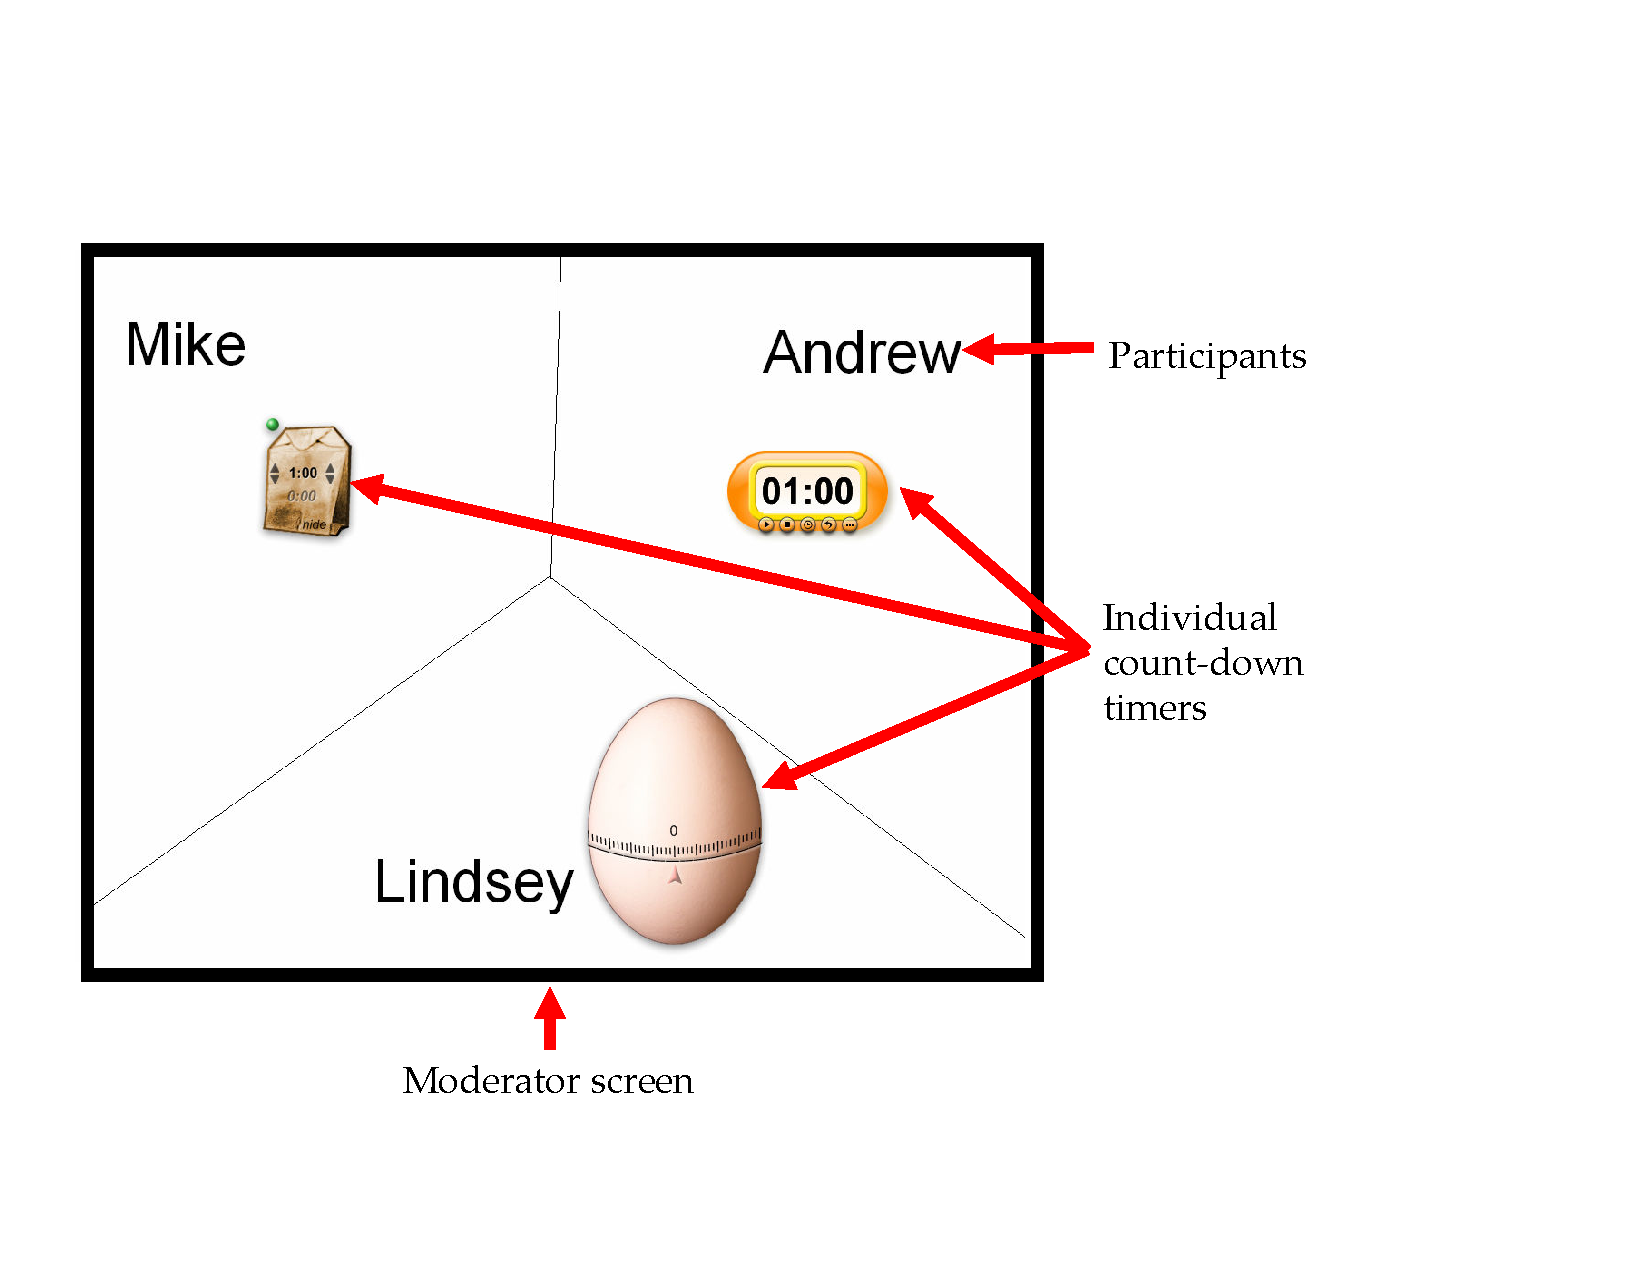
\includegraphics[width=1.00\textwidth]{Figures/Ch5/moderator.pdf}
	\caption{View of moderator display}
	\label{fig:moderator}
\end{figure}

\begin{center}
\color{blue}
(Text omitted for brevity)
\normalcolor
\end{center}


Each was simply a countdown timer with a default starting time, $t_{s}$. As they begin counting down, the amount of time remaining is visible. By clicking twice on any widget, it would reset and begin counting down again from $t_{s}$. The timers were manually reset by one of the teammates during the meeting whenever someone had an interaction. When any timer runs out, it would sound an alarm, designating that the meeting come to a halt until the non-active team member contributes to the conversation. The hypothesis was that, because the timers were visible to the entire team, each member would consciously make an effort to speak before their timer ran out and that no timer would actually buzz, although the rotation of speakers would greatly increase.

The moderator screen was displayed on a 32" LCD display that was positioned 6' from the center of a table where the group met. The layout is detailed in Figure \ref{fig:moderator_setup}. No video or audio conferencing was used -- all team members were local. The objective of the moderator is to support dialogue in meetings, regardless of whether the members are distributed or not. Audio was recorded of each meeting using Cubase software and an IBM laptop's internal microphone, which was placed in the center of the table so each participant could be heard. 

\begin{figure}[h]
	\centering
		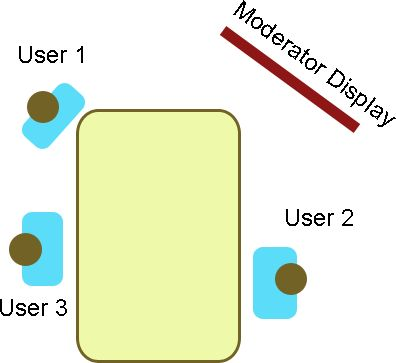
\includegraphics[width=.75\textwidth]{Figures/Ch5/moderator_setup.jpg}
	\caption{Layout of design meeting with moderator prototype}
	\label{fig:moderator_setup}
\end{figure}

\subsubsection{Procedure}

Three meetings were run to test the moderator. The subject of each was the same - our team brainstormed potential final products knowing the key lessons learned after our benchmarking. Three meetings were run in succession, each lasting 30 minutes. The intention of this was to eliminate any personal changes between meetings. For example, if Mike has a really bad day before coming in for a second meeting, he may be much less talkative than in the previous meeting, but not as a result of the moderator. The first meeting served as the control, and no moderator was used. The two subsequent meetings used the moderator with $t_{s}$ at 2 minutes and 1 minute.

The audio files were analyzed manually by playing back the audio recordings for each meeting and recording the length of each comment that every person made. Fifteen minutes of audio during the middle of each meeting was processed. The data are available in Appendix \ref{sec:Appendix1}. 

\subsection{CFP Lessons Learned}

\begin{remark}  \color{blue}
Ideally  there should be something among these findings that reflects back to the personas. Are there particular findings in light of the personas? Do the findings cause you to modify your personas?
\normalcolor \end{remark}

	Tactile sensation is an effective means of communicating contextual information. The messaging system delivered instant vibration between the two stations, helping preserve the flow of conversation without impeding it. Using the vibrations to alert the other users that you wanted to say something was a good way to make comments at the precise time you intended. The tactile devices were \textbf{easy to use} and the participants were encouraged to use them as they saw fit. We noticed that \textbf{vibrations were used most frequently to add emphasis} � to accompany laughter, to confirm agreement, offer praise for a good idea � and to interrupt the speaker. Interruptions consisted of calls for clarification on a point raised or disagreement with an opinion. Interrupting someone who is speaking can cause the speaker to lose his train of thought or become otherwise agitated. We noticed that \textbf{users preferred to send low speed vibrations} as a gentle interruption as a first attempt to get the speaker's attention. If the first few low speed vibrations did not stop the speaker, the high speed vibrations could be sent, and these usually registered right away. We observed that users reserved high speed vibrations for urgent or important messages. 
	
	
	The signals were mostly easy to detect, but it was \textbf{not always clear what those signals were trying to communicate}. Ambiguous or superfluous signals distracted the receiving user from the meeting and the confused user would ask, ''Did you just buzz me?'' or ''�Why did you buzz me?'' These confused questions would stall the meeting for everyone until the sender was revealed and was able to explain what they were trying to communicate. 
	
	Vibrations, however, were easily detectable despite loud side conversations, a party in a neighboring room, and constant distractions from people walking by. We attribute this to the fact that the tactile channel is uncrowded compared to the audio channel. In a loud environment it is difficult to pick out audio communication from Skype. Visual distractions make it difficult to focus on the laptop monitor. The tactile sensation rarely stimulated in a teleconference, thus making the slightest vibration very noticeable. 
	
	We tried two different vibrating interfaces, a vibrating pen and a vibrating wrist patch. The wrist patch was unanimously rejected by the participants because 1) the double stick tape that connected the patch to the user's skin was either too sticky and removed arm hair or not sticky enough after a few uses and would fall off, 2) was tethered to the power supply and restricted movement to the point where the hand with the patch was essentially stationary, 3) vibrations on your wrist are not comfortable, and 4) worry that the patch might give the user an electrical shock. The pen had a practical use, writing, and although the pen was connected to the power supply, the user was not, and the range of motion was adequate enough to write anywhere on the drawing space.
	
	We finally compared the tactile messaging conference to previous experiences with video conferencing and audio conferencing. These results are summarized in Appendix \ref{sec:Appendix1}.
	
		\begin{figure}[h] 
\centering
		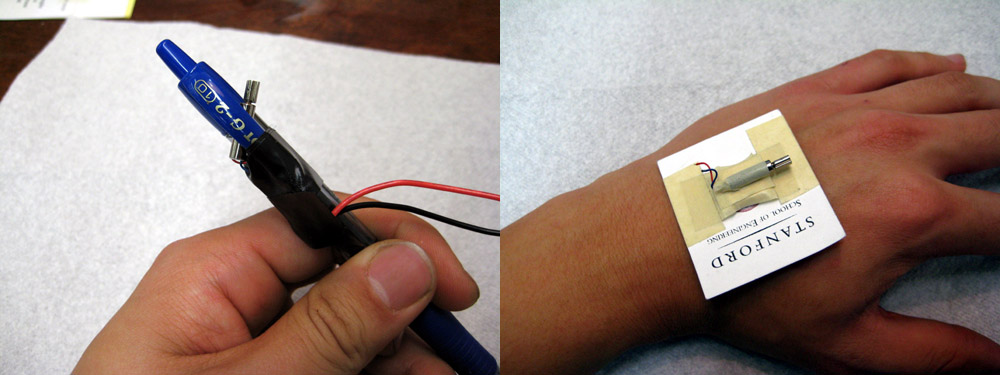
\includegraphics[width=0.8\textwidth]{Figures/Ch4/tactile_motor.jpg}
	\caption[Messaging station wires]{The orientation of the two tactile messaging stations. (Note: the wires connecting the patch to power supply are not in this photo)}
\end{figure}

	The tactile messaging critical function prototype was a success in that it definitively answered all the critical questions we asked ourselves before testing.
